\documentclass[a4paper,12pt]{article}
\usepackage[english]{babel}
\usepackage[utf8]{inputenc}
\usepackage{amsmath,amssymb}
 \usepackage{graphicx}
\usepackage{xcolor}
\usepackage{tabularx}
\usepackage{lipsum}    

\addtolength{\voffset}{-2cm} \addtolength{\textheight}{4cm}   
\addtolength{\hoffset}{-1cm} \addtolength{\textwidth}{2cm}
 
\begin{document}

\begin{center}
Sveučilište u Splitu\\
Prirodoslovno-matematički fakultet \\
Odjel za f\mbox{}iziku

\bigskip
\bigskip

\large{Programski alati u fizici}


\bigskip
\bigskip

\textbf{{\Large{Gibanje dvostrukog njihala}}}           
\end{center}
\begin{center}
\textbf{Jure Jerčić}\\
\
\end{center}
\begin{center}
Split, 8.6.2023.                                           
\end{center}

\section*{Sažetak}
Cilj ovoga rada bio je simulirati gibanje dvostrukog njihala (eng. \textit{double pendulum}) bez otpora zraka te izraditi animaciju gibanja. Jednadžbe ovog problema implentirane su u simulaciju gibanja dvostrukog njihala koristeći Eulerovu metodu u programskom jeziku Python, koristeći biblioteke NumPy i Matplotlib. Simulacijom i animacijom ovog problema vizualno je predočeno gibanje dvostrukog njihala čime se lako dobiva uvid u kaotičnost ovakvog gibanja te utjecaj sitnih odstupanja od početnih uvjeta na gibanje.


\section{Uvod}

Dvostruko njihalo fizički je objekt sastavljen od dva njihala koja su povezana jedno na drugo (Slika 1). Gornje njihalo fiksirano je u jednoj točki oko koje se giba, dok se donje njihalo giba oko gibajuće krajnje točke gornjeg njihala. Indeks $1$ odnosi se na gornje njihalo, a indeks $2$ na donje. Mase njihala su $m_1$ i $m_2$, duljine $l_1$ i $l_2$, a kutevi pod kojima su njihala položena u odnosu na $y$-os  iznose $\theta_1$ i $\theta_2$. Položaji masa koje promatramo kao materijalne točke na krajevima njihala su
$$x_1=l_1 \sin\theta_1, \quad y_1=-l_1\cos\theta_1,$$
$$x_2=x_1+l_2 \sin\theta_2, \quad y_2=y_1-l_2\cos\theta_2,$$ a prva derivacija položaja daje brzine
$$x_1^{'}=\theta_1^{'} l_1 \cos\theta_1, \quad y_1^{'}=\theta_1^{'}l_1\sin\theta_1,$$
$$x_2^{'}=x_1^{'}+\theta_2^{'}l_2 \cos\theta_2, \quad y_2^{'}=y_1^{'}+\theta_2^{'}l_2 \sin\theta_2,$$ dok je druga derivacija akcelaracija svake mase
$$x_1^{''}=-(\theta_1^{'})^{2} l_1 \sin\theta_1 + \theta_1^{''} l_1 \cos\theta_1, \quad y_1^{''}=(\theta_1^{'})^{2} l_1 \cos\theta_1 + \theta_1^{''} l_1 \sin\theta_1,$$
$$x_2^{''}=x_1^{''}-(\theta_2^{'})^{2} l_2 \sin\theta_2 + \theta_2^{''} l_2 \cos\theta_2, \quad y_2^{'}=y_1^{''}+(\theta_2^{'})^{2} l_2 \cos\theta_2 + \theta_2^{''} l_2 \sin\theta_2$$


\begin{figure}[h!]
\centering
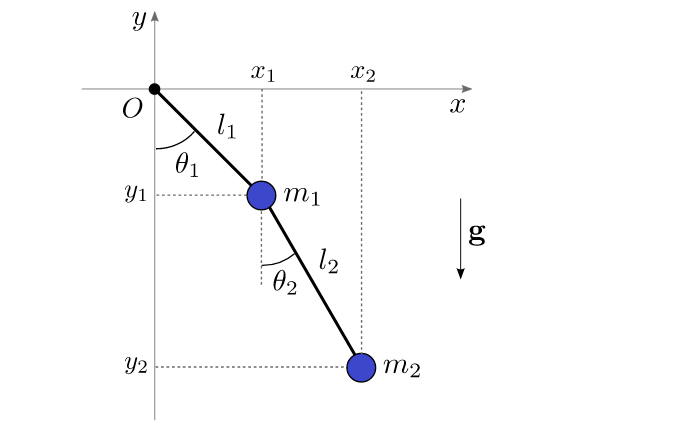
\includegraphics[width=7cm]{dp_fig1.png}
\caption{Skica dvostrukog njihala sa označenim pripadajućim veličinama. Preuzeto iz \cite{Slika1}. }
\end{figure}

Sile koje djeluju u sustavu su sile napetosti niti njihala $\vec{T_i}$ te gravitacijska sila $m_i\vec{g}$, dok je djelovanje otpora zraka zanemareno. Pozivajući se na drugi Newtonov zakon zapisujemo slijedeće jednadžbe za gornje i donje njihalo po $x$ i $y$ komponentama, redom:
$$m_1 x_1^{''} = -T_1\sin\theta_1+T_2\sin\theta_2,\quad m_1 y_1^{''} = T_1\cos\theta_1-T_2\cos\theta_2-m_1g$$
$$m_2 x_2^{''} = -T_2\sin\theta_2,\quad m_2 y_2^{''} = T_2\cos\theta_2-m_2g$$
Sređivanjem koristeći \cite{Jedn} dobivama konačne izraze za kutne brzine i akceleracija njihala:
$$\theta_1^{'}=\omega_1$$
$$\theta_2^{'}=\omega_2$$
$$\omega_1^{'}=\frac{-g(2m_1+m_2)\sin\theta_1-m_2g\sin(\theta_1-2\theta_2)-2\sin(\theta_1-\theta_2)m_2(\omega_2^{2} l_2+\omega_1^{2} l_1\cos(\theta_1-\theta_2))}{l_1(2m_1+m_2-m_2\cos(2\theta_1-2\theta_2))}$$
$$\omega_2^{'}=\frac{2\sin(\theta_1-\theta_2)(\omega_1^{2}l_2(m_1+m_2)+g(m_1+m_2)\cos\theta_1+\omega_2^{2}l_2m_2\cos(\theta_1-\theta_2))}{l_2(2m_1+m_2-m_2\cos(2\theta_1-2\theta_2))}$$
Dobivene jednadžbe možemo implementirati u kod koji će simulirati gibanje dvostrukog njihala i napraviti animaciju istoga.
\section{Diskusija i rezultati}
Za simulacija ovog problema korišten je programski jezik Python s pripradajućim bibliotekama NumPy i Matplotlib. Problem je riješen objektno-orijentiranim pristupom programiranju kreiranjem klase $DoublePendulum$ koja kao ulazne parametre prima prethodno definirane veličine, odnosno mase $[kg]$, duljine $[m]$, početne kutove otklona $[\deg]$ i početne kutne brzine  $[\deg s^{-1}]$ gornjeg i donjeg njihala. Klasi su također zadani vremenski parametri $T$ i $dt$ koji redom označavaju trajanje simulacije i vremenski korak između numeričkih operacija.
\\
U metodi $\_\_init\_\_$ inicijaliziranje su sve početne vrijednosti te su definirane nove veličine koje se u kodu koriste za riješavanje zadanog problema. Kutne veličine su iz stupnjeva pretvorene u radijane koristeći numpy metodu $radians()$. Brojač vremena $t$ postavljen je na $0 s$. Također su definirana polja u koja se spremaju $x$ i $y$ koordinate gibajućih masa njihala. Inicijalizirani su i animacijski elemnti odnosno varijable $pend1$ i $pend2$ koja predstavljaju gornje i donje njihalo te brojač vremena u animaciji $timer$ i $animation$ koji poziva animacijsku funkciju
\\
Metoda $diff\_solve$ kao ulazne parametre prima kutne veličine za oba njihala te vraća njihove derivacije koje su numerički riješene koristeći formule navedene u Uvodu. Izračunate se vrijednosti koriste dalje u kodu prilikom simuliranja gibanja i računanja koordinata u metodi $\_\_move$. U metodi $\_\_move$ koristi se Eulerova metoda za numeričko rješavanje relevantnih jednadžbi ovoga problema polazeći od početnih vrijednosti zadanih prilikom kreiranja klase. Ovom se metodom problem dijeli na vrlo male vremenske intervale trajanja $dt s$ pri čemu se u svakom koraku jednostavno može izračunati nove vrijednosti kinematičkih veličina i tako dok vremenski brojač $t$ ne postigne zadano vrijeme trajanja simulacije gibanja $T$ kada se zaustavlja animacija. U ovoj se metodi koristeći izračunate nove vrijednosti kutnih veličina računaju koordinate njihala. U svakom se koraku povećava i brojač $timer$ za iznos $dt$ te se novoizračunate koordinate njihala dodjeljuju dvodimenzijonalnim elemetima $pend1$ i $pend2$. 
Pomoću metode $animate$ definira se animacijski okvir pomoću $matplotlib$ biblioteke. Prostor prikazan u animaciji kvadratno je omeđen te je sustav dvostrukog njihala postavljen u ishodište oko kojega se giba. Animacija se postiže pozivanjem funkcije $FuncAnimation$ koja u zadanom animacijskom prostoru $fig$ prikazuje gibanje dvostrukog njihala pozivajući se na funkciju, odnosno prethodno definiranu privatnu metodu $\_\_move$. 
\\
Za početne uvjete $l_1 = 1\, m,\, m_1 = 1\, kg,\, \theta_1 = 120^\circ,\, \omega_1 = 0,\,l_2 = 1\, m,\, m_2 = 1\, kg,\, \theta_2 = 90^\circ,\, \omega_2 = 0,\, T = 5\, s$ i $dt = 0.0075\,s$ pokrenuta je simulacija gibanja danog dvostukog njihala. Simulacija je uspješno pokrenuta te grafičkim prikazom putanje donjeg njihala, odnosno donje mase $m_2$ dobivamo uvid u kaotičnost gibanja ovakvog sustava. Da bi se demostrirala osjetljivost ovakvog sustava, ali i koda na početne uvjete promatrana je i putanja kada vremenski korak $dt$ iznosi $0.0085\, s$. Usporedbom ovih dviju putanja za dane vremenske korake (Slika 2, sredina i desno) vidi se kako one izgedaju dosta slično, ali ipak postoje značajnija odstupanja koja postaju jasnija odmakom vremena. Sitne promjene u početnim uvjetima značajno utječu gibanje ovakvog kaotičnog sustava. Kada se vremenski korak vrati na početni $dt = 0.0075\,s$ te se kut otklona gornjeg njihala poveća na $\theta_1 = 122^\circ$ promatranjem putanje vidi se da je simulacija, odnosno gibanje njihala vrlo osjetljivo i na promjenu fizikalnih veličina, odnosno početnih uvjeta gibanja, za fiskni $dt$. I animacija i fizikalni sustav osjetljivi su na početne parametre. Mala promjena na samom početku gibanja može imati za uzrok značajna međusobna odstupanja putanja danih sustava, što opet potvrđuje kaotičnost ovahvih sustava i veliku osjetljivost na početne uvjete (Slika 2, lijevo).
\begin{figure}[h!]
	\centering
	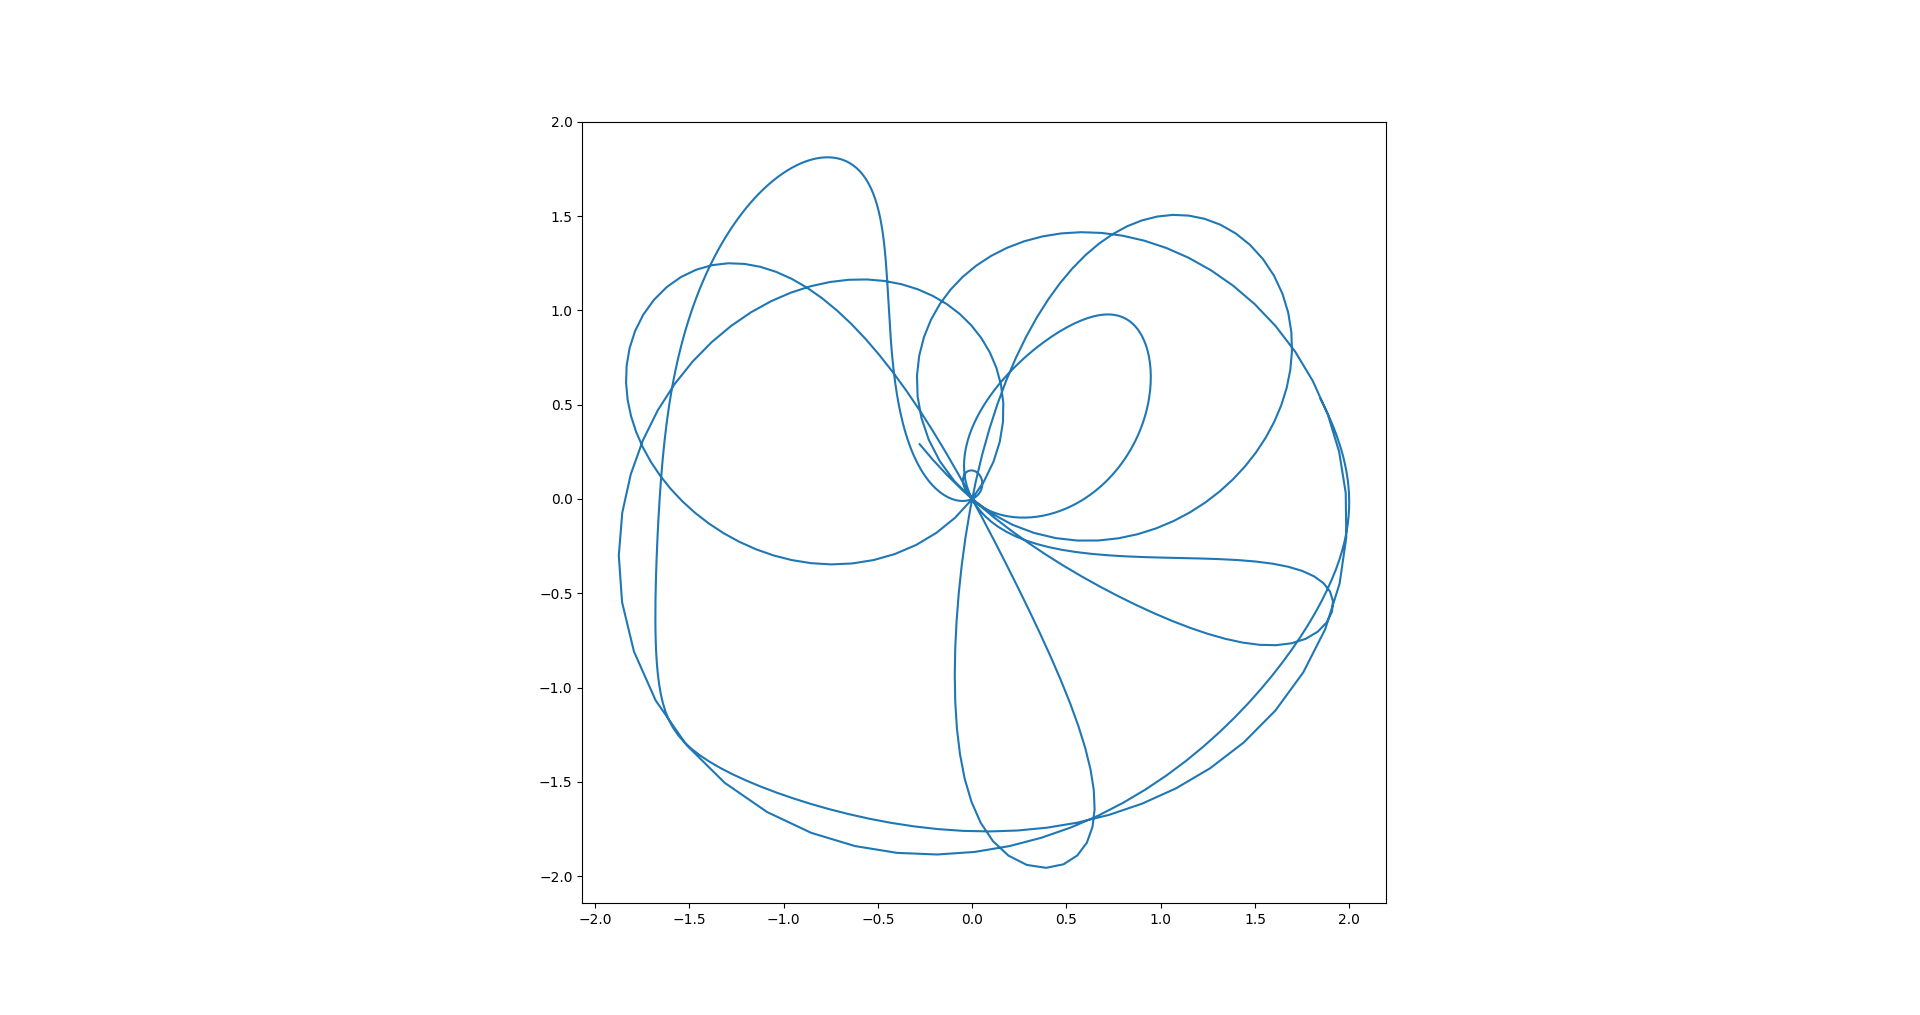
\includegraphics[width=5.1cm]{trajectory122.png}
	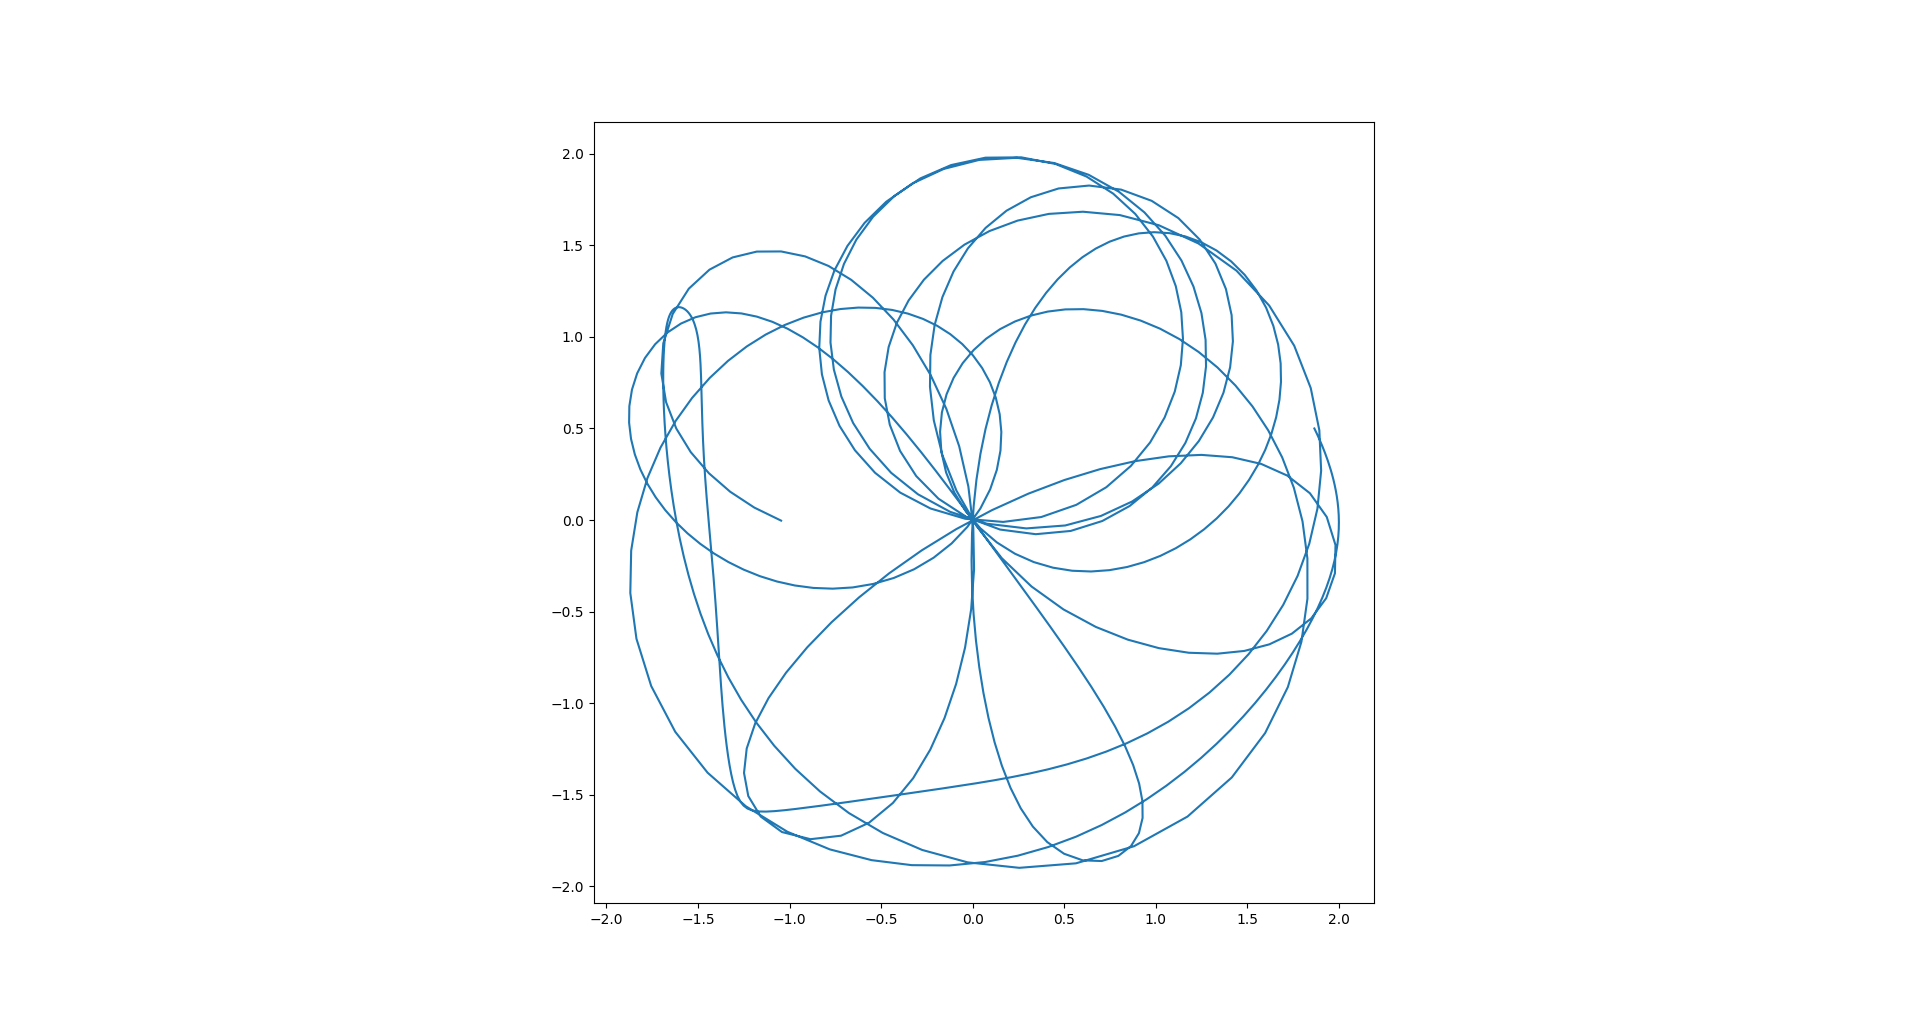
\includegraphics[width=5.1cm]{trajectory.png}	
	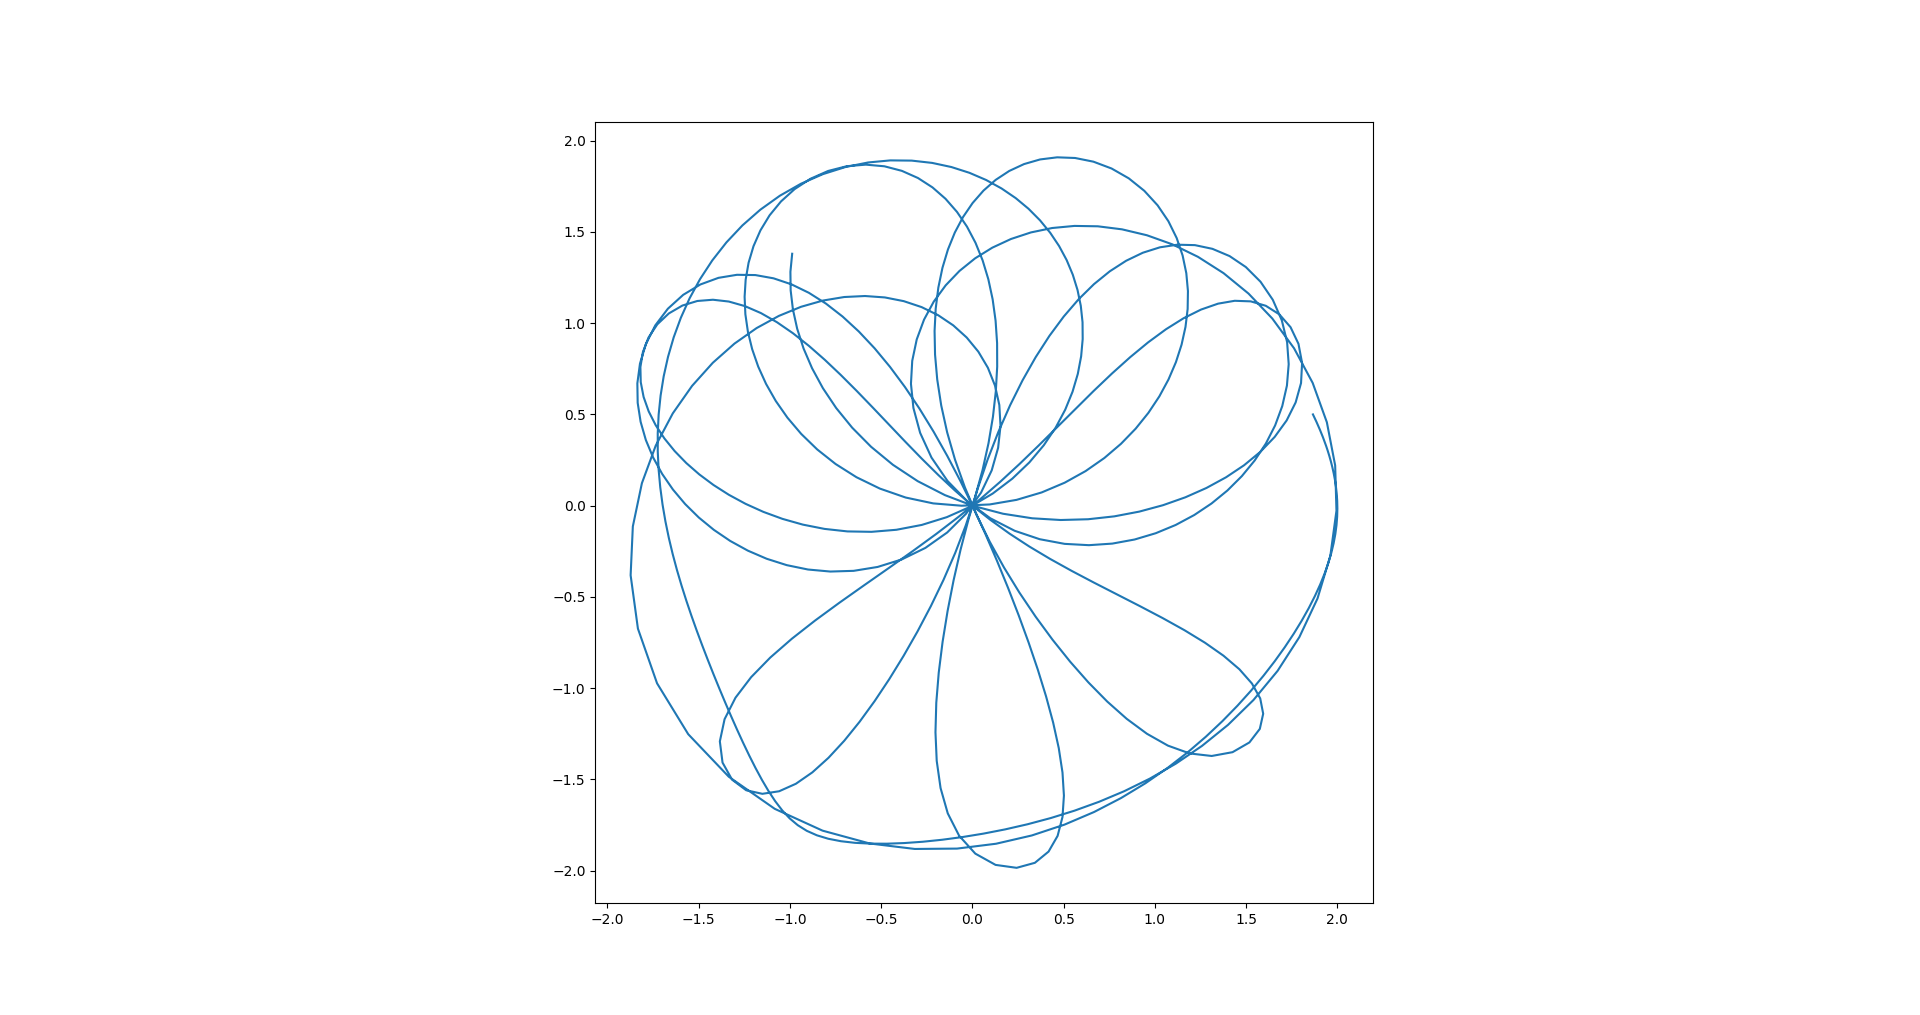
\includegraphics[width=5.1cm]{trajectory85.png}

	\caption{Putanje dvostrukog njihala za zadane parametre kada je: $(dt = 0.0075\,s,\,\theta_1 = 122^\circ)$ (lijevo), $(dt = 0.0075\,s,\,\theta_1 = 120^\circ)$ (sredina) i $(dt = 0.0085\,s,\,\theta_1 = 120^\circ)$ (desno)}
\end{figure}
\section{Zaključak}

Razvojem modula $DoublePendulum.py$ simulirano je i animirano gibanje dvostrukog njhala koristeću Eulerovu metodu. Problem dvostrukog njihala demostrira kaotičnost i osjetljivost problema na početne uvjete. Simuliranjem koda za različite vrijednosti koje su relativno slične uočena su znatna međusobna odstupanja te je na taj način potvrđen kaotični karakter ovog problema. Kako bi se postigle preciznije simulacije kod bi se mogao unaprijediti korištenjem neke naprednije metode numeričkog rješavanja jednadžbi, iako je ovakvo rješenje relativno precizno, posebno za manje vremenske korake. 


\begin{thebibliography}{9}
\bibitem{Slika1}{https://physics.stackexchange.com/questions/724082/kinetic-energy-of-double-pendulum}
\bibitem{Jedn}{https://web.mit.edu/jorloff/www/chaosTalk/double-pendulum/double-pendulum-en.html}


\end{thebibliography}

\end{document}


%%%%%%%%%%%%%%%%%%%%%%%%%%%%%%%%%%%%%%%%
%    Izmijenjeno od:        Uzorak dokumenta za seminar iz moderne fizike, 2019.          %
%                            Mislav Cvitković, Split, svibanj 2019.                          %
%%%%%%%%%%%%%%%%%%%%%%%%%%%%%%%%%%%%%%%%
